\documentclass[a4paper,UTF8]{article}
\usepackage{ctex}
\usepackage[margin=1.25in]{geometry}
\usepackage{color}
\usepackage{graphicx}
\usepackage{amssymb}
\usepackage{amsmath}
\usepackage{amsthm}
\usepackage{tcolorbox}
\usepackage{enumerate}
\usepackage{hyperref}
\usepackage{pythonhighlight}
%\usepackage[thmmarks, amsmath, thref]{ntheorem}
\theoremstyle{definition}
\newtheorem*{solution}{Solution}
\newtheorem*{prove}{Proof}
\usepackage{multirow}              

\setlength{\evensidemargin}{.25in}
\setlength{\textwidth}{6in}
\setlength{\topmargin}{-0.5in}
\setlength{\topmargin}{-0.5in}
% \setlength{\textheight}{9.5in}
%%%%%%%%%%%%%%%%%%此处用于设置页眉页脚%%%%%%%%%%%%%%%%%%
\usepackage{fancyhdr}                                
\usepackage{lastpage}                                           
\usepackage{layout}                                             
\footskip = 10pt 
\pagestyle{fancy}                    % 设置页眉                 
\lhead{2020年春季}                    
\chead{机器学习导论}                                                
% \rhead{第\thepage/\pageref{LastPage}页} 
\rhead{作业三}                                                                                               
\cfoot{\thepage}                                                
\renewcommand{\headrulewidth}{1pt}  			%页眉线宽,设为0可以去页眉线
\setlength{\skip\footins}{0.5cm}    			%脚注与正文的距离           
\renewcommand{\footrulewidth}{0pt}  			%页脚线宽,设为0可以去页脚线

\makeatletter 									%设置双线页眉                                        
\def\headrule{{\if@fancyplain\let\headrulewidth\plainheadrulewidth\fi%
		\hrule\@height 1.0pt \@width\headwidth\vskip1pt	%上面线为1pt粗  
		\hrule\@height 0.5pt\@width\headwidth  			%下面0.5pt粗            
		\vskip-2\headrulewidth\vskip-1pt}      			%两条线的距离1pt        
	\vspace{6mm}}     								%双线与下面正文之间的垂直间距              
\makeatother  

%--

%--
\begin{document}
\title{机器学习导论\\习题三}
\author{171830635, 俞星凯, yuxk@smail.nju.edu.cn}
\maketitle


\section*{学术诚信}

本课程非常重视学术诚信规范,助教老师和助教同学将不遗余力地维护作业中的学术诚信规范的建立。希望所有选课学生能够对此予以重视。\footnote{参考尹一通老师\href{http://tcs.nju.edu.cn/wiki/}{高级算法课程}中对学术诚信的说明。}

\begin{tcolorbox}
	\begin{enumerate}
		\item[(1)] 允许同学之间的相互讨论,但是{\color{red}\textbf{署你名字的工作必须由你完成}},不允许直接照搬任何已有的材料,必须独立完成作业的书写过程;
		\item[(2)] 在完成作业过程中,对他人工作(出版物、互联网资料)中文本的直接照搬(包括原文的直接复制粘贴及语句的简单修改等)都将视为剽窃,剽窃者成绩将被取消。{\color{red}\textbf{对于完成作业中有关键作用的公开资料,应予以明显引用}};
		\item[(3)] 如果发现作业之间高度相似将被判定为互相抄袭行为,{\color{red}\textbf{抄袭和被抄袭双方的成绩都将被取消}}。因此请主动防止自己的作业被他人抄袭。
	\end{enumerate}
\end{tcolorbox}

\section*{作业提交注意事项}
\begin{tcolorbox}
	\begin{enumerate}
		\item[(1)] 请在LaTeX模板中第一页填写个人的学号、姓名、邮箱;
		\item[(2)] 本次作业需提交该pdf文件、问题4可直接运行的源码(.py文件)、问题4的预测结果(.csv文件),将以上三个文件压缩成zip文件后上传。注意:pdf、预测结果命名为“学号\_姓名”(例如“181221001\_张三.pdf”),源码、压缩文件命名为“学号”,例如“181221001.zip”;
		\item[(3)] 未按照要求提交作业,提交作业格式不正确,{\color{red}\textbf{作业命名不规范}},将会被扣除部分作业分数;
		\item[(4)] 本次作业提交截止时间为{\color{red}\textbf{4月23日23:55:00}}。除非有特殊情况(如因病缓交),否则截止时间后不接收作业,本次作业记零分。
	\end{enumerate}
\end{tcolorbox}

\newpage
\section{[20pts] Decision Tree I}
\begin{enumerate}[(1)]
	\item \textbf{[5pts]} 试分析使用“最小训练误差”作为决策树划分选择的缺陷。
	\item \textbf{[5pts]}  树也是一种线性模型,考虑图(\ref{img})所示回归决策树,$X_1,X_2$均在单位区间上取值,$t_1,t_2,t_3,t_4$满足$0<t_1<t_3<1,0<t_2,t_4<1$,试绘制出该决策树对于特征空间的划分。假设区域$R_i$上模型的输出值为$c_i$,试用线性模型表示该决策树。
	\begin{figure}[htbp]
		\centering
		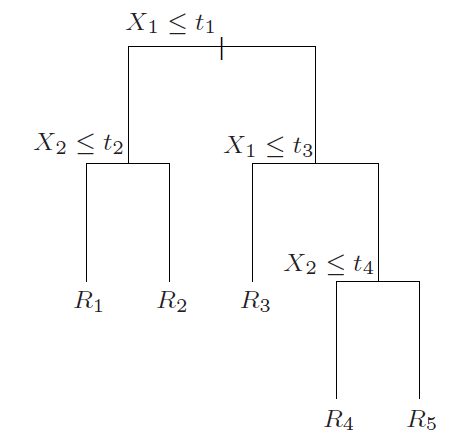
\includegraphics[width=.4\textwidth]{figure/regression_tree.png} %1.png是图片文件的相对路径
		\caption{回归决策树} %caption是图片的标题
		\label{img} %此处的label相当于一个图片的专属标志,目的是方便上下文的引用
	\end{figure}
	\item \textbf{[10pts]} 对于回归树,我们常采用平方误差来表示回归树对于训练数据的预测误差。但是找出平方误差最小化准则下的最优回归树在计算上一般是不可行的,通常我们采用贪心的算法计算切分变量$j$和分离点$s$。CART回归树在每一步求解如下优化问题
	$$\min _{j, s}\left[\min _{c_1} \sum_{x_{i} \in R_{1}(j, s)}\left(y_{i}-c_{1}\right)^{2}+\min _{c_{2}} \sum_{x_{i} \in R_{2}(j, s)}\left(y_{i}-c_{2}\right)^{2}\right]$$
	其中$R_1(j,s)=\{\boldsymbol{x}|x_j\leq s\},R_2(j,s)=\{\boldsymbol{x}|x_j>s\}$。试分析该优化问题表达的含义并给出变量$j,s$的求解思路。
\end{enumerate}

\begin{solution}
	~\\
	\begin{enumerate}[(1)]
		\item 
		使用“最小训练误差”作为划分选择,为了尽可能正确分类训练样本,结点划分过程将不断重复,有时会造成决策树分支过多,导致过拟合。
		\item 
		\[
		y=\begin{cases}
		&R1,\quad 0\leq X_1\leq t_1, 0\leq X_2\leq t_2\\
		&R2,\quad 0\leq X_1\leq t_1, t_2<X_2\leq 1\\
		&R3,\quad t_1<X_1\leq t_3\\
		&R4,\quad t_3<X_1\leq 1, 0\leq X_2\leq t_4\\
		&R5,\quad t_3<X_1\leq 1, t_4<X_2\leq 1
		\end{cases}
		\]
		\begin{figure}[htbp]
			\centering
			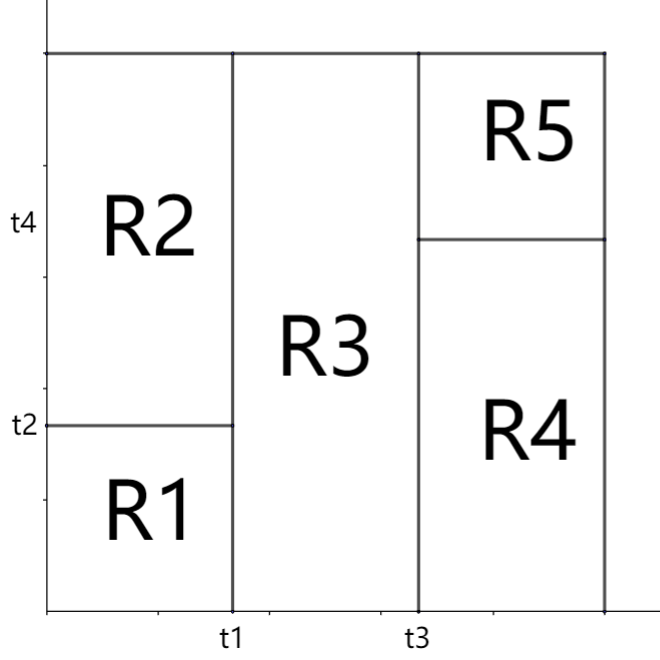
\includegraphics[width=.4\textwidth]{figure1.png}
			\caption{特征空间划分}
		\end{figure}
		\item 
		选择第$j$个维度和分割点$s$,根据数据在第$j$个维度上的取值$x_j$与$s$的大小关系,将数据集分成两部分$R_1$和$R_2$。对$R_k$中的数据预测$c_k(k=1,2)$,这样$R_k$中数据的平方误差和$\sum\limits_{x_{i} \in R_{k}(j, s)}(y_{i}-c_{1})^2$,从而我们优化问题
		\[\min _{j, s}\left[\min _{c_1} \sum_{x_{i} \in R_{1}(j, s)}\left(y_{i}-c_{1}\right)^{2}+\min _{c_{2}} \sum_{x_{i} \in R_{2}(j, s)}\left(y_{i}-c_{2}\right)^{2}\right]\]
		容易得到$c_k$是$R_k$中数据标签$y_i$的均值
		\[c_k=ave(y_i|x_i\in R_k),\quad k=1,2\]
		$j,s$的优化可以通过下面方法得到
		\begin{enumerate}[(a)]
			\item 
			对于固定的$j$,将数据集上不同的$x_j$依次作为切分点$s$,计算代价函数,选择使得代价函数最小的$x_j^*$作为切分点$s$。
			\item 
			遍历所有的维度,分别调用上面步骤,选择使得代价函数最小的$j$及其对应的$s$。
		\end{enumerate}
	\end{enumerate}
\end{solution}

\section{[25pts] Decision Tree II}

\begin{enumerate}[(1)]
	\item \textbf{[5pts]} 对于不含冲突数据(即特征向量相同但标记不同)的训练集,必存在与训练集一致(即训练误差为$0$)的决策树。如果训练集可以包含无穷多个数据,是否一定存在与训练集一致的深度有限的决策树?证明你的结论。(仅考虑单个划分准则仅包含一次属性判断的决策树)
	\item \textbf{[5pts]} 考虑如表\ref{train data for tree}所示的人造数据,其中“性别”、“喜欢ML作业”是属性,“ML成绩高”是标签。请画出使用信息增益为划分准则的决策树算法所有可能的结果。(需说明详细计算过程)
	\begin{table}[h]
		\caption{训练集}
		\label{train data for tree}
		\centering
		\begin{tabular}{cccc}
			\hline 
			编号 & 性别 & 喜欢ML作业 & ML成绩高 \\ 
			\hline 
			1 & 男 & 是 & 是 \\ 
			2 & 女 & 是 & 是 \\ 
			3 & 男 & 否 & 否 \\ 
			4 & 男 & 否 & 否 \\ 
			5 & 女 & 否 & 是 \\ 
			\hline 
		\end{tabular}
	\end{table}
	\item \textbf{[10pts]} 考虑如表\ref{validation data for tree}所示的验证集,对上一小问的结果基于该验证集进行预剪枝、后剪枝,剪枝结果是什么?(需给出详细计算过程)
	\begin{table}[h]
		\caption{验证集}
		\label{validation data for tree}
		\centering
		\begin{tabular}{cccc}
			\hline 
			编号 & 性别 & 喜欢ML作业 & ML成绩高 \\ 
			\hline 
			6 & 男 & 是 & 是 \\ 
			7 & 女 & 是 & 否 \\ 
			8 & 男 & 否 & 否 \\ 
			9 & 女 & 否 & 否 \\ 
			\hline 
		\end{tabular}
	\end{table}
	\item \textbf{[5pts]} 比较预剪枝、后剪枝的结果,每种剪枝方法在训练集、验证集上的准确率分别为多少?哪种方法拟合能力较强?
\end{enumerate}

\begin{solution}
	~\\
	\begin{enumerate}[(1)]
		\item 
		不一定存在。考虑这样一个数据集:输入$x\in \mathbb{N}$,输出$y\in {0,1}$,当$x$是奇数时,$y=1$,当$x$是偶数时,$y=0$。对于这个数据集,不存在与包含无穷多个数据的训练集一致的深度有限的决策树。
		\item 
		\begin{multline*}
		Gain(D,\text{性别})=-(\frac35\log_2\frac35+\frac25\log_2\frac25)+[\frac35(\frac13\log_2\frac13+\frac23\log_2\frac23)+\frac25(\frac12\log_2\frac12+\frac12\log_2\frac12)]=0.02\\
		Gain(D,\text{喜欢ML作业})=-(\frac35\log_2\frac35+\frac25\log_2\frac25)+[\frac25(\frac22\log_2\frac22+\frac02\log_2\frac02)+\frac35(\frac13\log_2\frac13+\frac23\log_2\frac23)]=0.42
		\end{multline*}
		因为属性“喜欢ML作业”的信息增益大,所以根据喜欢ML作业,将数据集$D$划分为$D^1(\text{喜欢})$和$D^2(\text{不喜欢})$。
		$D_1$中的样本属于同一类别,无需划分。
		\[
		Gain(D^2,\text{性别})=-(\frac13\log_2\frac13+\frac23\log_2\frac23)+[\frac23(\frac02\log_2\frac02+\frac22\log_2\frac22)+\frac13(\frac11\log_2\frac11+\frac01\log_2\frac01)]=0.92
		\]
		根据性别,将$D^2$划分为$D^3(\text{男生,不喜欢})$和$D^4(\text{女生,不喜欢})$。\\
		预测$D^1$和$D^4$中的学生成绩高,$D^3$中的学生成绩不高。
		\begin{figure}[htbp]
			\centering
			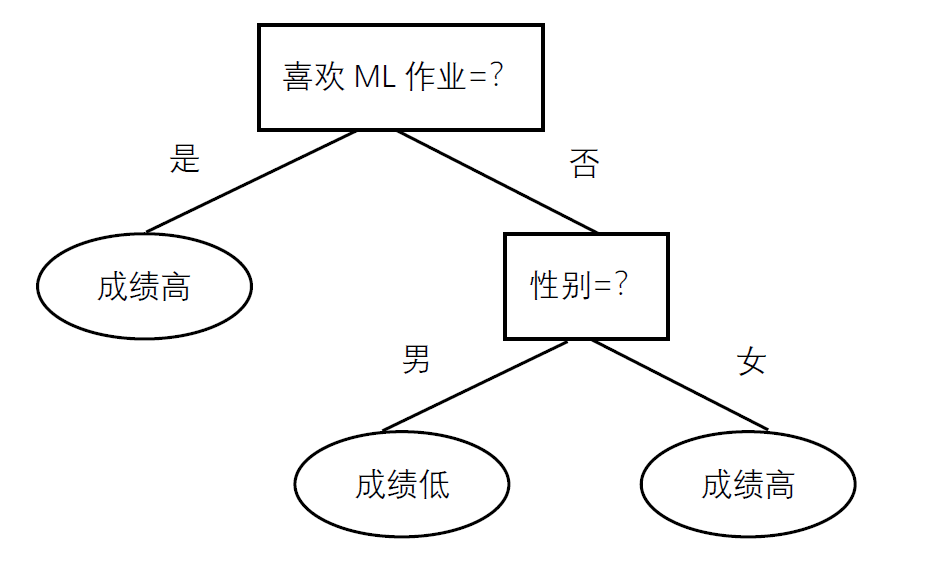
\includegraphics[width=.4\textwidth]{figure2.png}
			\caption{决策树}
		\end{figure}
		\item 
		预剪枝过程如下:\\
		对$D^1$基于信息增益选择属性“喜欢ML作业划分”,划分前训练集中ML成绩高的样例多,因此预测成绩高,这在验证集中的精度为$\frac14=25\%$。划分后对$D^1$预测成绩高,对$D^2$预测成绩不高,验证集精度为$\frac34=75\%$,所以需要划分。\\
		对$D^2$选择属性“性别”,划分前验证集精度$75\%$,划分后对$D^3$预测成绩不高,对$D^4$预测成绩高,验证集精度为$\frac14=25\%$,因此禁止划分。\\
		\begin{figure}[htbp]
			\centering
			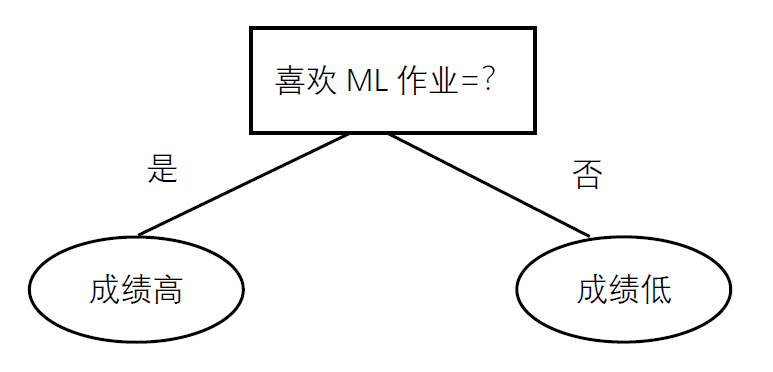
\includegraphics[width=.4\textwidth]{figure3.png}
			\caption{预剪枝结果}
		\end{figure}
		后剪枝过程如下:\\
		生成完整决策树,验证集精度为$\frac14=25\%$。若将性别决策移除,则对于不喜欢ML作业的样例预测成绩不高,验证集精度$\frac34=75\%$,于是决定剪枝。\\
		再考虑将喜欢ML作业决策移除,则对于所有样例预测ML成绩高,验证集精度$\frac14=25\%$,决定不剪枝。\\
		\begin{figure}[htbp]
			\centering
			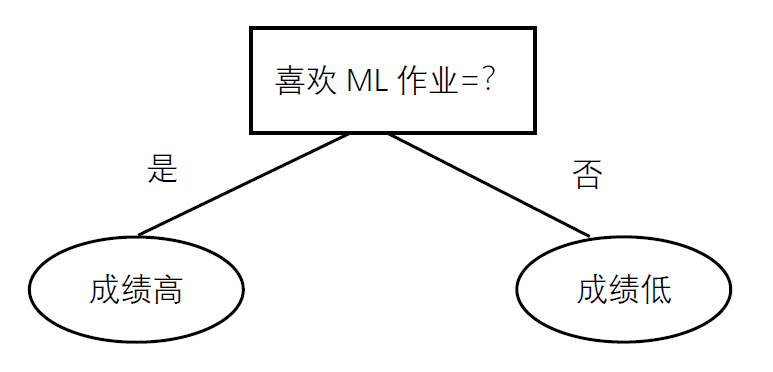
\includegraphics[width=.4\textwidth]{figure3.png}
			\caption{后剪枝结果}
		\end{figure}
		\item 
		预剪枝的训练集精度$80\%$,验证集精度$75\%$,后剪枝的训练集精度$80\%$,验证集精度$75\%$。在这个例子中拟合能力一样,但是一般来说后剪枝拟合能力更强。
	\end{enumerate}
\end{solution}

\section{[25pts] SVM with Weighted Penalty}
考虑标准的SVM优化问题如下(即课本公式(6.35)),
\begin{equation}
\label{eq-svm}
\begin{split}
\min_{\mathbf{w},b,\xi_i}& \quad \frac{1}{2} \lVert \mathbf{w} \rVert^2 + C\sum_{i=1}^m\xi_i\\
\text{s.t.}&  \quad y_i(\mathbf{w}^\mathrm{T}\mathbf{x}_i + b)\geq 1-\xi_i\\
& \quad \xi_i \geq 0, i = 1,2,\cdots,m.
\end{split}
\end{equation}

注意到,在\eqref{eq-svm}中,对于正例和负例,其在目标函数中分类错误或分对但置信度较低的“惩罚”是相同的。在实际场景中,很多时候正例和负例分错或分对但置信度较低的“惩罚”往往是不同的,比如癌症诊断等。

现在,我们希望对负例分类错误(即false positive)或分对但置信度较低的样本施加$k>0$倍于正例中被分错的或者分对但置信度较低的样本的“惩罚”。对于此类场景下,

(1) \textbf{[10pts]} 请给出相应的SVM优化问题。

(2) \textbf{[15pts]} 请给出相应的对偶问题及KKT条件,要求详细的推导步骤。

\begin{solution}此处用于写解答(中英文均可)
	\begin{enumerate}[(1)]
		\item 
		修改SVM优化问题
		\begin{align*}
		\min_{w,b,\xi_i}&\quad\frac{1}{2}\lVert w\rVert^2+C\sum_{i=1}^m(\frac{k+1}2-\frac{k-1}2y_i)\xi_i\\
		\text{s.t.}&\quad y_i(w^Tx_i + b)\geq 1-\xi_i\\
		&\quad\xi_i\geq 0,i=1,2,\cdots,m.
		\end{align*}
		\item 
		引入拉格朗日乘子得到拉格朗日函数
		\[
		L(w,b,\alpha,\xi,\mu)=\frac{1}{2}\lVert w\rVert^2+C\sum_{i=1}^m(\frac{k+1}2-\frac{k-1}2y_i)\xi_i+\sum_{i=1}^m\alpha_i(1-\xi_i-y_i(w^Tx+b))-\sum_{i=1}^m\mu_i\xi_i
		\]
		令$L(w,b,\alpha,\xi,\mu)$对$w,b,\xi$的偏导为零可得
		\begin{align*}
		w&=\sum_{i=1}^m\alpha_iy_ix_i,\\
		0&=\sum_{i=1}^m y_ix_i,\\
		C&=(\alpha_i+\mu_i)/(\frac{k+1}2-\frac{k-1}2y_i)
		\end{align*}
		代入原问题得到对偶问题
		\begin{align*}
		\max_\alpha&\quad\sum_{i=1}^m\alpha_i-\frac12\sum_{i=1}^m\sum_{j=1}^m\alpha_i\alpha_j y_i y_j x_i^T x_j\\
		\text{s.t.}&\quad \sum_{i=1}^m \alpha_iy_i=0,\\
		&\quad 0\leq\alpha_i\leq C(\frac{k+1}2-\frac{k-1}2y_i),\quad i=1,2,\cdots,m.
		\end{align*}
		KKT条件要求
		\[
		\left\{
		\begin{aligned}
		&\alpha_i\geq0,\quad\mu_i\geq0,\quad\xi_i\geq0\\
		&y_if(x_i)-1+\xi_i\geq0\\
		&\alpha_i(y_if(x_i)-1+\xi_i)=0\\
		&\mu_i\xi_i=0
		\end{aligned}
		\right.
		\]
	\end{enumerate}
\end{solution}

\section{[30 pts] 编程题, Linear SVM}
\textbf{请结合编程题指南进行理解}

SVM转化成的对偶问题实际是一个二次规划问题,除了SMO算法外,传统二次规划方法也可以用于求解对偶问题。求得最优拉格朗日乘子后,超平面参数$\mathbf{w,b}$可由以下式子得到:
\begin{equation}
\mathbf{w} = \sum_{i=1}^m \alpha_i y_i x_i
\end{equation}
\begin{equation}
\mathbf{b} = \frac{1}{|S|}\sum_{s\in S} (y_s-\sum_{i\in S}\alpha_i y_i x_i^T x_s)
\end{equation}
请完成以下任务:
\begin{enumerate}[(1)]
	\item \textbf{[5pts]} 使用QP方法求解训练集上的SVM分类对偶问题(不考虑软间隔情况)。
	\item \textbf{[10 pts]} 手动实现SMO算法求解上述对偶问题。
	\item \textbf{[15 pts]} 对测试数据进行预测,确保预测结果尽可能准确。
\end{enumerate}

\begin{solution}
	~\\
	\begin{enumerate}[(1)]
	\item 
	使用python的cvxopt库求解QP问题,核心求解过程如下:
\begin{python}
	P = matrix((y @ y.T) * (X @ X.T) + np.diag(np.full(m, 1e-7)))
	q = matrix(-np.ones(m))
	G = matrix(-np.eye(m))
	h = matrix(np.zeros(m))
	A = matrix(y.T)
	b = matrix(0.0)
	solvers.options['show_progress'] = False
	sol = solvers.qp(P, q, G, h, A, b)
\end{python}
	于是可以得到对偶变量$\alpha$,进而求出$w$和$b$:
\begin{python}
	alpha = np.array(sol['x'])
	w = X.T @ (alpha * y)
	indice = np.ravel(alpha > 1)
	b = np.mean(y[indice] - X[indice] @ w)
\end{python}
	cvxopt求出的解在训练集上精度为81\%。
	\item 
	首先计算距离每个样本最远的异类样本,这里充分利用了数组广播:
\begin{python}
	D = np.sum(np.square(X[np.newaxis,:,:] - X[:,np.newaxis,:]), -1)
	D = y @ y.T * D
	D = np.argmin(D, 1)
\end{python}
	然后迭代优化,先计算KKT违背程度:
\begin{python}
	w = X.T @ (alpha * y)
	indice = np.ravel(alpha > 0.01)
	b = np.mean(y[indice] - X[indice] @ w)
	err = np.ravel(y * (X @ w + b) - 1)
	err[indice] **= 2
	err[~indice & (err >= 0)] = 0
	err[~indice & (err < 0)] **= 2
\end{python}
	再确定需要优化的$\alpha_i$和$\alpha_j$,根据自己推导的公式更新:
\begin{python}
	i = np.argmax(err)
	j = D[i]
	c = alpha[i] * y[i] + alpha[j] * y[j] - alpha.T @ y
	p = np.sum(alpha * y * X @ X[i].T)
	q = np.sum(alpha * y * X @ X[j].T)
	r = X[i] @ X[j].T
	t = 1 - y[i] * y[j] - y[i] * p + y[i] * q + y[i] * c * r
	t /= 2 * r
	alpha[i] = max([0, t])
	alpha[j] = c * y[j] - y[i] * y[j] * alpha[i]
\end{python}
	最后得到的结果在训练集上精度为80\%到82\%。
	\item 
	尝试使用核技巧,修改训练代码,先求核矩阵:
\begin{python}
	D = np.exp(np.sum(np.square(X[np.newaxis,:,:] - X[:,np.newaxis,:]), -1) \
			/ (-2 * sigma ** 2))
	P = matrix(y @ y.T * D + np.diag(np.full(m, 1e-7)))
\end{python}
	同样也要修改测试代码,发现核技巧结果不好。\\
	尝试对某些特征取倒数,最好结果是82.5\%。
\begin{python}
	d = {}
	for i in range(1, 6):
		for j in combinations(range(5), i):
			X_temp = X_train.copy()
			X_temp[:, j] = 1 / X_temp[:, j]
			w, b = QP(X_temp, y_train)
			y_pred = np.sign(X_temp @ w + b)
			d[j] = np.mean(y_pred == y_train)
	print("the accuracy using inverse of feature:", max(d.items(), key=lambda x: x[1]))
\end{python}
	类似尝试对某些特征取平方和指数,结果都在81\%左右。
	\end{enumerate}
\end{solution}
\end{document}